%==========================================================================================

\documentclass[10pt]{article}

%==========================================================================================

\usepackage[utf8]{inputenc}
\usepackage[brazil]{babel}
\usepackage[T1]{fontenc}
\usepackage{amsmath}
\usepackage{amsfonts}
\usepackage{mathrsfs}
\usepackage{amssymb}
\usepackage{graphicx}
\usepackage{geometry, calc, color, setspace}
\usepackage{indentfirst}
\usepackage{wrapfig}
\usepackage{boxedminipage}
\usepackage{enumerate}
\usepackage{float}
\usepackage[hang]{caption}
\usepackage{paralist}
\usepackage{comment}
\usepackage{icomma}
\usepackage{rotating}
\usepackage{multirow}

\usepackage{array}
\newcolumntype{C}[1]{>{\centering\let\newline\\\arraybackslash\hspace{0pt}}m{#1}}

\usepackage[abnt-substyle=UFLA,abnt-emphasize=bf,abnt-etal-list=3,abnt-and-type=e]{abntcite}

\newcommand{\HRule}{\noindent\rule{\linewidth}{0.2mm}}

\usepackage{mathpazo}                         % tem suporte matemático
\usepackage[scaled=0.85]{beramono}            % usa esta nos verbatins [scaled=0.9]

\def\distnumber{2.3em}

%==========================================================================================

\author{Walmes Marques Zeviani\footnote{Doutorando em Estatística e
Experimentação Agropecuária, DEX/UFLA. Professor do Departamento de Estatística
- UFPR. Contato: walmes@ufpr.br.}}

%==========================================================================================


\title{Uma parametrização de um modelo não linear para inferência sobre o nível
de dano econômico da desfolha no algodoeiro}
\date{}

\begin{document}

\maketitle

\begin{abstract}
O efeito da desfolha sobre a qualidade e produtividade das culturas é
informação fundamental para definir estratégias de manejo, como
intensidade e frequência de pastejo e colheita até o estabelecimento
de níveis de dano econômico de forma a auxiliar decisões sobre o
controle de pragas desfolhadoras. Para a cultura do algodão, assim
como para outras tantas, a redução da produção pela desfolha pode ser
representada por uma função não linear monótona não
crescente. Diversos modelos podem satisfazer essa restrição, no
entanto, existe a preocupação de inferir sobre o nível de dano
econômico, $\vartheta_q$, pelo ajuste de um modelo. Dados de
produção-desfolha do algodoeiro em função do estágio fenológico são
considerados para inferir sobre o nível de dano econômico com os
seguintes objetivos: 1) propor uma parametrização de modelo que
representasse o parâmetro, 2) avaliar parametrizações alternativas por
meio de medidas de não linearidade, 3) aplicar inferência baseada em
verossimilhança, 4) selecionar um modelo para descrever a relação
entre produção e desfolha do algodoeiro em função do estágio
fenológico. O modelo reparametrizado apresentou menores medidas de não
linearidade nos estágios fenológicos com pronunciada relação não
linear. Nos restantes, as medidas de curvatura, as correlações dos
estimadores e os gráficos de perfil de verossimilhança indicaram que
um sub-modelo deveria ser considerado.\\
\newline
\noindent {Palavras-chave}: Interpretação de parâmetros. Verossimilhança. Método delta. Curvatura. \emph{Gossypium hirsutum}.

\end{abstract}

\section{INTRODUÇÃO}

Em condições de campo, as culturas estão sujeitas à perdas de área
foliar por diferentes causas, dentre elas o pastejo e a colheita
periódica das folhas, o ataque de insetos desfolhadores e de doenças
que causam sua queda ou necrose, as chuvas de granizo e a própria
senescência natural são as mais frequentes.  Uma desfolha
significativa reduz o potencial fotossintético e, dependendo da
intensidade e fase de crescimento da planta, ocasiona prejuízos à
produção \cite{Painter1981,Klubertanz1996}.  Algumas doenças e pragas,
fitotoxicidade de pesticidas ou adubos, granizo e certas injúrias
mecânicas são eventos comuns que causam desfolha em áreas de cultivo
de algodão e que podem prejudicar a produção e qualidade do produto
dessa cultura \cite{Silva2012a}.

\newpage
\section{MODELO}

A relação monótona não crescente entre produção e desfolha é a
informação preliminar considerada para elaborar um modelo. Dentre as
funções matemáticas que atendem à essa imposição, tem-se o modelo
potência, chamado de modelo Herschel-Bulkley por
\citeonline{Cheng1992}, como opção,
\begin{equation}
 f(x) = \theta_0-\theta_1 x^{\theta_2}, \qquad x\geq 0.
\end{equation}
A desfolha, $x$ (adimensional), assume valores entre 0 e 1.  A
produção normal, com unidade de medida representada por Y, prevista
sem haver desfolha é representada pelo parâmetro $\theta_0$ (Y), ou
seja, $f(0) = \theta_0$.  A redução na produção normal ao ocorrer uma
desfolha total é $\theta_1\geq 0$, ou seja, $f(0)-f(1) = \theta_1$.  O
parâmetro adimensional $\theta_2>0$ é um parâmetro de forma dessa
relação, que é côncava se $\theta_2>1$, convexa se $0<\theta_2<1$ e
linear se $\theta_2=1$. É conveniente reescrever o modelo considerando
a transformação $\theta_2 = \exp\{\theta_c\}$ uma vez que a função
exponencial é positiva e que isso não compromete a interpretação do
modelo em $\theta_2$ que é apenas um parâmetro de forma.  Dessa forma,
\begin{equation}\label{eq-modelo}
 f(x) = \theta_0-\theta_1 x^{\exp\{\theta_c\}}, \qquad x\geq 0,
\end{equation}
é uma função côncava para $\theta_c>0$, convexa para $\theta_c<0$ e
linear quando $\theta_c=0$ (Figura \ref{fig:herschel}).

\newpage
\section{MATERIAL E MÉTODOS}

\begin{figure}[!b]
\begin{center}
 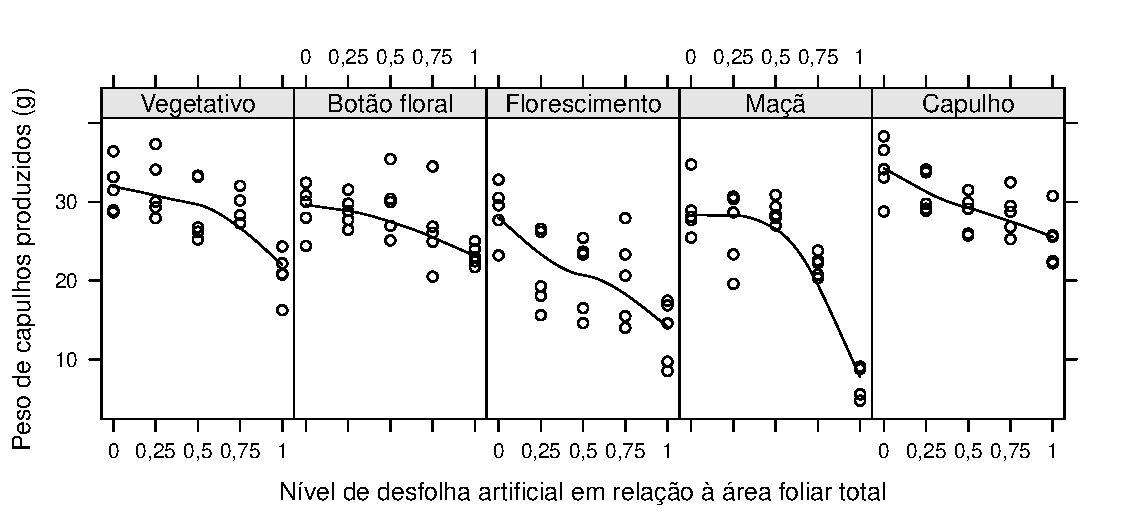
\includegraphics[width=\textwidth]{../figuras/previsu.pdf} 
\end{center}
\caption{Peso de capulhos produzidos (g) em cada estágio fenológico
  como função dos níveis de desfolha artificial. Curvas suaves entre
  os pontos representam as tendências centrais}\label{previsu}
\end{figure} 

Os dados considerados para ajuste do modelo são de um experimento, em
casa de vegetação, com a cultura do algodão (\emph{Gossypium
  hirsutum}). As unidades experimentais foram 2 plantas por vaso para
registro da produção total de pluma com caroço (g).  Os fatores
estudados foram o nível de desfolha artificial (0, 25, 50, 75 e
100\%), feita com tesoura em cada uma das folhas da planta conforme
tais níveis, combinados com o estágio fenológico no qual a desfolha
foi realizada (vegetativo, presença de botão floral, florescimento,
presença de maçã e presença de capulho). O delineamento completamente
ao acaso foi utilizado com cinco repetições, perfazendo $5\times
5\times 5 = 125$ unidades experimentais.  O experimento foi realizado
nas dependências da Universidade Federal de Grande Dourados no ano
agrícola de 2007. Mais informações disponíveis em
\citeonline{Silva2012a}.  Na Figura \ref{previsu} tem se o diagrama de
dispersão dos valores observados de peso de capulhos produzidos (g) em
cada estágio fenológico como função dos níveis de desfolha.

\newpage
\section{RESULTADOS E DISCUSSÃO}

Os ajustes dos modelos aos dados convergiram para os cinco estágios
fenológicos, considerando o máximo de 50 interações.  Valores iniciais
baseados na inspeção do diagrama de dispersão foram considerados
(Figura \ref{previsu}).  As estimativas dos parâmetros comuns,
$\theta_0$ e $\theta_1$, foram idênticas, em termos pontuais e
intervalares, nas duas parametrizações, como de fato devem ser pois
ambas parametrizações descrevem o mesmo modelo (Tabela
\ref{tb-estimic}). Percebeu-se um resultado alarmante para o estágio
de florescimento, no qual os intervalos de confiança para $\theta_0$ e
$\theta_1$ foram demasiado amplos, superando inclusive a amplitude
média de variação dos dados, de aproximadamente 5 g para cima e para
baixo, ao redor da curva de tendência.

\newpage
\section{CONCLUSÕES}

O propósito da reparametrização foi representar o nível de dano
econômico no modelo. As parametrizações foram comparadas com relação
aos métodos disponíveis para fazer inferência sobre o nível de dano
econômico. A inferência baseada em verossimilhança foi mais adequada
no sentido de auxiliar a seleção de modelos. Além do mais,
verificou-se que as medidas de curvatura e inspeção da matriz de
covariâncias das estimativas também são úteis no processo de seleção
de modelos. Nos estágios com pronunciada relação linear para
produção-desfolha, o modelo reparametrizado apresentou melhores
propriedades inferenciais.  O algodoeiro responde de forma
diferenciada à desfolha em cada estágio fenológico.

\newpage
\addcontentsline{toc}{section}{\hspace*{\distnumber}REFERÊNCIAS}
\begin{center}
\section*{REFERÊNCIAS} 
\end{center}


% Use isso descomentado durante edição.
% Quando concluir a Tese, comente iss e use
% o código do bloco abaixo.
\begin{singlespace}
\renewcommand\refname{}
\begin{flushleft}
\bibliography{bibtese2}
\end{flushleft}
\end{singlespace}

%% Em cap3nls-corrigido.bbl foi feita correção manual de
%% algumas referências como por exemplo as citações
%% de Dissertação e Tese.
%% Então deixa-se de usar o arquivo cap3nls.bbl gerado
%% automaticamente pelo abntcite, mas isso é só ao final.
% \begin{singlespace}
% \begin{flushleft}
% \renewcommand\refname{}
% \vspace*{-1.5cm}
% \input{cap3nls-corrigido.bbl}
% \end{flushleft}
% \end{singlespace}

\section{Anexos}

\begin{singlespace}
\noindent{{ANEXO A:$\,\,$} Código R reproduzível correspondente ao
ajuste do modelo potência reparametrizado para inferência sobre o
nível de dano econômico da desfolha no algodoeiro.
Disponível online
em: \texttt{http://www.leg.ufpr.br/\~{}walmes /TESE/anexoDESF.R}}
\end{singlespace}
\noindent \rule[4mm]{\textwidth}{0.1ex}
\begin{small}
\linespread{0.7}
\vspace{-1cm}
\input{../scripts/anexoDESF.R}
\noindent \rule[4mm]{\textwidth}{0.1ex}
\end{small}

\begin{minipage}{\textwidth}
\noindent{{ANEXO B:$\,\,$} Peso de capulhos produzido (g) ao final do
ciclo a cada duas plantas de algodão em função do nível de desfolha
artifical e estágio fenológico.}
\begin{center}
 \input{../tabelas/anexotabDESF.txt}
\end{center}
\end{minipage}

\end{document}

%==========================================================================================
